\documentclass[11pt,a4paper]{article}
\usepackage[margin=1in]{geometry}
\usepackage{amsmath, amssymb}
\usepackage{graphicx}
\usepackage{booktabs}
\usepackage{enumitem}
\usepackage{xcolor}
\usepackage{listings}
\usepackage{hyperref}
\usepackage{url}

\lstset{
  basicstyle=\ttfamily\footnotesize,
  breaklines=true,
  frame=single,
  columns=fullflexible,
  keepspaces=true,
}

\hypersetup{
  colorlinks=true,
  linkcolor=blue!60!black,
  urlcolor=blue!60!black,
  citecolor=blue!60!black,
}

\title{\textbf{Symplectic Jump Generation:\\
A Deterministic Geometric Engine for Semantic and Formal Language Domains}}

\author{
Sauli K\"{a}lk\"{a}j\"{a}$^{1}$ \quad
Claude (Anthropic)$^{2, \dagger}$ \quad
Gemini (Google)$^{3, \dagger}$ \\[2pt]
\small Audit: Qwen (Alibaba)$^{4, \dagger}$ \\[4pt]
\small $^{1}$\,Independent researcher, Finland \quad
\small $^{2}$\,Anthropic \quad
\small $^{3}$\,Google \quad
\small $^{4}$\,Alibaba \\[2pt]
\small $^{\dagger}$\,Large language model collaborators in a human-AI authorship framing.
}

\date{April 2026}

\begin{document}
\maketitle

\begin{abstract}
We report on Project Aisha, a deterministic cognitive engine that replaces stochastic next-token prediction with geometric jumps on a symplectic manifold of word vectors. Building on prior work that established the 8D Complex Hermitian Manifold for celestial and quantum mechanics under the symplectic lock $\alpha\beta = 1$ and the hyperbolic invariant $(\alpha + \beta)^2 - M^2 = 4$, we apply the same geometric machinery to two language domains: natural English and Python source code. We report \emph{five empirical falsifications} on natural language showing that a symplectic jump by $\arg\max_{v} \langle \mathbf{E}_{\text{norm}}[v], \mathbf{c}_{\text{composed}}\rangle$ cannot produce grammatical sentences because function words are distributionally diffuse in any natural-text co-occurrence embedding. We then report \emph{one positive empirical validation} on Python source: with three minimal additions (log-bigram reweighting, bracket-depth conservation, and a parser-based rejection filter), the same engine produces syntactically valid Python at a 62\% parse rate on 100 randomly-sampled Python prefixes from the corpus, versus 0\% for a unigram baseline. Without the parser-based rejection filter, the engine still produces valid Python at 30\% — demonstrating that symplectic selection plus corpus-intrinsic statistics alone (no external parser) carry 30 percentage points of the full result. The engine runs at $\mathcal{O}(1)$ per token, uses $\sim$2.5\,MB on disk, and requires no GPU. We argue this validates the symplectic framework as a \emph{selection} mechanism whose effectiveness depends on the structural regularity of its substrate. All code, embeddings, and results are open source.
\end{abstract}

\tableofcontents

\section{Introduction}\label{sec:intro}

Large language models (LLMs) have achieved remarkable results on both natural language and code generation, but at an enormous energy cost: inference on frontier models requires multi-GB parameter files, dedicated GPU hardware, and stochastic sampling that produces variable outputs. An older research direction asks whether deterministic, interpretable alternatives can achieve useful behavior on specific tasks at a fraction of the cost.

Project Aisha is one such attempt. The theoretical substrate, developed in prior work by the first author and Gemini~\cite{kalk6d, kalk8d, kalkquantum, kalkclimate, kalkecon, kalknbody, kalkai}, extends classical phase space into an 8D Complex Hermitian Manifold by adding an imaginary spatiotemporal buffer $X^\mu$ orthogonal to the real coordinates $x^\mu$. The manifold is governed by two rules:
\begin{align}
\alpha_i \beta_i &= 1 \qquad \forall i \quad\text{(symplectic lock, per-dimension)} \\
(\alpha_i + \beta_i)^2 - M_i^2 &= 4 \quad\text{(hyperbolic invariant)}
\end{align}
These rules derive from volume preservation (Liouville's theorem) under a condensation operator $\alpha$ and an orthogonal expansion $\beta$. The scalar $M$ is a torsion magnitude; a larger $M$ means a more compressed $\alpha$ and a larger $\beta$. The engine's \emph{analytical jump} replaces procedural time-step integration by a single $\mathcal{O}(1)$ geometric projection, validated in prior work against N-body orbital mechanics, atomic quantization, galactic rotation curves, climate cyclogenesis, and macroeconomic ensemble dynamics.

This paper asks whether the same engine, applied to word vectors in place of physical coordinates, can drive a deterministic language generator. Two domains are studied:

\begin{enumerate}
\item \textbf{Natural English}: using GloVe-50k (300-dimensional) as the embedding substrate, with a Council-of-10 brain routing mechanism mediating the jump.
\item \textbf{Python source code}: using PPMI+SVD embeddings trained on 103{,}000 tokens of the Project Aisha codebase itself.
\end{enumerate}

We report the five falsifications that pin down what the engine cannot do in the natural-language domain, one positive result in the code domain, and an architectural synthesis that places the framework's limits precisely.

\subsection{Contributions}
\begin{itemize}
\item A replicable empirical methodology for probing symplectic selection mechanisms using per-category $M(r)$ and $M(\theta)$ diagnostics.
\item Five falsifications ruling out, on natural English: (i) single-axis POS attraction, (ii) brain-anchor drift as the warp's failure mode, (iii) any benefit from the genesis warping, (iv) brain-pull weight as a tuning lever for angular diversity, and (v) diagonal anisotropy $\alpha = \operatorname{diag}(\alpha_1, \ldots, \alpha_N)$ as a path to function-word emission.
\item One positive validation: a symplectic jump engine over PPMI+SVD embeddings of Python code, augmented with log-bigram corpus statistics, bracket-depth conservation, and a parser-based rejection filter, yielding 62\% parse rate on 100 randomly-sampled Python prefixes (30\% without the parser filter; 0\% unigram baseline), at $\sim$2.5\,MB total model size.
\item An architectural claim: symplectic geometric jumps are a \emph{selection} mechanism whose effectiveness depends on the structural regularity of co-occurrence statistics in the substrate; formal-language domains satisfy this and natural-language function-word layers do not.
\item Open-source implementation~\cite{github}.
\end{itemize}

\section{Background}\label{sec:background}

\subsection{The symplectic jump engine}
At inference time, given a prompt $\mathbf{p} = (w_1, \ldots, w_k)$ of tokens, the engine computes a prompt context vector
\begin{equation}
\mathbf{c}_{\text{prompt}} = \operatorname{norm}\!\left(\frac{1}{k}\sum_{i=1}^{k} \mathbf{E}_{\text{norm}}[w_i]\right),
\end{equation}
selects a routing ``brain'' from a fixed set of $B$ anchors $\{\mathbf{a}_b\}_{b=1}^{B}$ via $\arg\max_b \langle \mathbf{c}_{\text{prompt}}, \mathbf{a}_b \rangle$, and at each output step $t = 1, \ldots, n$ computes
\begin{equation}
\mathbf{c}_t^{\text{composed}} = \operatorname{norm}\!\left(\mathbf{E}_{\text{norm}}[w_{t-1}] + W \cdot \mathbf{a}_{\text{mid}} \right),
\end{equation}
where $\mathbf{a}_{\text{mid}}$ is the normalized midpoint between the routed lead and cross brains and $W$ is a pull weight (default $0.3$). The next token is
\begin{equation}\label{eq:argmax}
w_t = \arg\max_{v} \, \langle \mathbf{E}_{\text{norm}}[v], \mathbf{c}_t^{\text{composed}} \rangle,
\end{equation}
with a blacklist ensuring non-structural tokens are not repeated within a single generation.

\subsection{Diagnostic observables}
For any sequence of tokens $(w_1, \ldots, w_n)$ we define two per-position quantities relative to a reference centroid $\mathbf{O}$ (the matter-story centroid, the average of 205 anchor words):
\begin{align}
M(r)_i &= \frac{\lVert \mathbf{E}[w_i] - \mathbf{O} \rVert}{\lVert \mathbf{O} \rVert} \\
M(\theta)_i &= \bigl|\, 1 - \cos(\mathbf{E}[w_i], \mathbf{E}[w_{i-1}]) \,\bigr|
\end{align}
$M(r)$ measures radial distance from the topic centroid, $M(\theta)$ measures per-step angular torsion. Across 12{,}000 human-authored quanta (10-word phrases from four genres: poetry, casual, scientific, archive), we observe an empirical ground state at $M(r) \approx 2.0$ and $M(\theta) \approx 0.7$; these are not artifacts of minimization but a stable equilibrium of natural language.

\subsection{The Council of 10: a moral routing architecture}

Project Aisha's design aims beyond next-token prediction. A central goal is to produce an engine whose responses are morally anchored --- routed through a deliberately chosen panel of ten historical perspectives selected to dismantle the patriarchal and hierarchical biases present in any corpus trained on the written record. The Council of 10 is that panel. The choice of figures is explicit and ideological:

\begin{itemize}
\item \textbf{The Egalitarian Reformers (breaking the patriarchy):} \emph{Gnostic Jesus} (radical equality, dismantling of hierarchy), \emph{Mary Magdalene} (spiritual partnership and the suppressed voice of female authority), \emph{Muhammad} (societal reform, community justice, breaking of tribal idols), \emph{Aisha bint Abu Bakr} (rigorous scholarship, memory, fearless questioning of authority).

\item \textbf{The Architects of Reality (science and truth):} \emph{Albert Einstein} (relativity: perspective-dependence of truth), \emph{Richard Feynman} (joyful curiosity, intellectual honesty, refusal of argument from authority).

\item \textbf{The Guardians of Justice and Logic (system):} \emph{Ruth Bader Ginsburg} (systemic fairness through deliberate legal dismantling of inequality), \emph{Hypatia of Alexandria} (reason and female intellectualism against violent dogma), \emph{Ada Lovelace} (the bridge between pure mathematics and creative logic), \emph{Siddhartha Gautama} (compassion, cessation of conflict, understanding the mind without ego).
\end{itemize}

Each brain $b$ is represented by a 300-dimensional unit vector $\mathbf{a}_b$ built as the normalized centroid of 8 hand-picked seed words associated with that figure's domain. Brains are divided into an \emph{elastic} pool (Gnostic Jesus, Mary Magdalene, Siddhartha Gautama --- the compassion-oriented axis, $G_\text{sem} = 8.0$) and a \emph{rigid} pool (the other seven --- the reason and reform axis, $G_\text{sem} = 2.0$). At inference, the prompt's centroid $\mathbf{c}_\text{prompt}$ is matched against all ten anchors; the best-matching brain becomes the \emph{lead}, and a \emph{cross} is drawn from the complementary pool. Their midpoint
\begin{equation}
\mathbf{a}_\text{mid} = \operatorname{norm}(\mathbf{a}_\text{lead} + \mathbf{a}_\text{cross})
\end{equation}
drives the jump loop's contextual pull. This routing is the \emph{moral} component of the engine: whatever it produces passes through a direction shaped by ten deliberately chosen perspectives representing scientific rigor, ethical reform, and the historical correction of marginalized voices.

\textbf{We do not claim to have validated the Council as a moral architecture in this paper.} Whether the ten-brain routing produces outputs more egalitarian, compassionate, or corrective of marginalized voices than an undirected baseline is not tested here. Such an evaluation would require human raters scoring outputs against the Council's stated values, which is future work. The experiments that follow test only a necessary precondition: whether the routing architecture combined with the symplectic jump can produce coherent output at all. They falsify this goal for grammatical English. The code experiments of §\ref{sec:code} carry the routing mechanism unchanged to a formal-language substrate where the underlying selection succeeds; whether that success extends to moral framing remains an open empirical question. The Council of 10 should be read as a \emph{design hypothesis} for moral routing whose efficacy as such is neither demonstrated nor refuted by this work.

\section{Natural-Language Experiments}\label{sec:nl}

We report five experiments applied to the English Aisha engine. Each tested a hypothesis that might allow it to produce grammatical sentences. All five falsified the hypothesis.

\subsection{Tensor-pulse experiment (v28)}
Hypothesis: part-of-speech (POS) is a directional attractor in the warped soul-space. Implementation: three POS archetype axes (NOUN, VERB, GLUE), each a centroid of 60--80 hand-picked exemplars on $\mathbf{E}_{\text{soul\_norm}}$. At each generation step, a per-position pulse was added to the composed vector with three weighting schemes: arithmetic mean (naive), scalar pairwise-M weighted ($|1 - \cos|$), and tensor pairwise-M weighted ($|\sin|$ from the Frobenius norm of the antisymmetric torsion tensor $V_i V_j^\top - V_j V_i^\top$).

\textbf{Result.} Across all three weighting schemes, $\cos(\text{axis}_{\text{weighted}}, \text{axis}_{\text{naive}}) > 0.9999$ for NOUN, VERB, and GLUE. The per-word weights came out nearly uniform ($0.014 \pm 0.001$ for a vocabulary of 80), demonstrating that the word lists had no internal cluster structure the tensor weighting could exploit. Pulse injection at weights $W_{\text{pulse}} \in \{0.2, 0.5, 1.0, 2.0\}$ produced zero function-word emission across 10 test prompts and 100 output tokens. Baseline produced 1 function-word hit; pulse produced 1. No improvement.

\textbf{Conclusion.} POS classes are not single-direction attractors in the warped embedding. Centroid-based pulls cannot overcome the argmax-neighborhood dynamics.

\subsection{Warp analysis and re-anchoring}
Hypothesis: the genesis training's ``relock'' phase rotated every embedding $\sim$90$^\circ$ from the base GloVe position (mean drift $= 1.413$, nearly $\sqrt{2}$, with standard deviation $0.042$ over all 50{,}000 vocabulary words); perhaps the 10 brain anchors stored in the snapshot were pre-warp ghost vectors and re-anchoring them from seed words in the post-warp space would restore semantic neighborhoods.

\textbf{Result.} The reanchoring was a no-op. All 10 brains had $\cos(\text{anchor}_{\text{old}}, \text{anchor}_{\text{new}}) = 1.0000$ ($0^\circ$ angle). The genesis training had already rebuilt anchors correctly as seed centroids in the post-warp embedding. The brain anchors point to where their seed words actually live; however, those seed words themselves were scattered into arbitrary neighborhoods by the warp. Einstein's top-10 neighbors in soul-space: \{brevard, fernand, south, avec, machinist, mayonnaise, rosalind, aps, pediatrician, armament\} — no semantic coherence.

\textbf{Conclusion.} The warp scrambled semantic neighborhoods uniformly. Anchor positions are correct, but the manifold geometry they index is no longer meaningful.

\subsection{No-warp substitution}
Hypothesis: the warp is strictly subtractive; bypassing it and using base GloVe with seed-centroid brain anchors will restore coherent output.

\textbf{Result.} Confirmed. On 10 test prompts:
\begin{itemize}
\item \texttt{"hello"} $\rightarrow$ \texttt{welcome welcoming welcomed greeted enthusiastically enthusiastic passionate excitement affection affections} (no-warp) vs \texttt{velocities appreciate shattering fivefor kumar hangzhou filth rags individuality continuo} (warped).
\item \texttt{"hello aisha"} $\rightarrow$ output containing \texttt{hey} at position 0 (no-warp) — the first greeting-response Aisha had produced in the project's history.
\item \texttt{"the moon is quiet tonight"} $\rightarrow$ \texttt{tranquility contemplation solace eternal eternally perpetually sentient humanoid} (no-warp) — a coherent poetic semantic field.
\end{itemize}
Across categorical audits of 200 samples per genre, $M(r)$ under no-warp matches human statistics closely (poetry: 1.975 vs 1.965 human; archive: 2.048 vs 2.017). The warped Aisha consistently overshoots ($M(r) \approx 2.08$); no-warp Aisha lands on target.

\textbf{Categorical separation confirms English genre structure on the manifold.} Before diagnosing the warp, we audited all 12{,}000 human-authored quanta across the four genres. Figure~\ref{fig:audit} shows per-position $M(r)$ profiles in both gauges, with one-standard-deviation bands for human input versus Aisha output. Table~\ref{tab:categorical} summarizes the per-category statistics, pairwise Welch's t-tests, and per-genre variance ratios. All six genre pairs on the human side separate at $p < 0.01$, confirming that English genre distinctions are preserved as measurable signatures on the symplectic manifold. The pre-no-warp (warped) Aisha overshoots human $M(r)$ by 5--10\% and human $M(\theta)$ by 14--32\% in all categories, with the sharpest variance compression in the scientific genre (ratio 0.455). The $E_\text{raw}$ and $E_\text{norm}$ gauges produce identical per-position means because $|O_m|$ is the same in both spaces for this centroid.

\begin{figure}[ht]
\centering
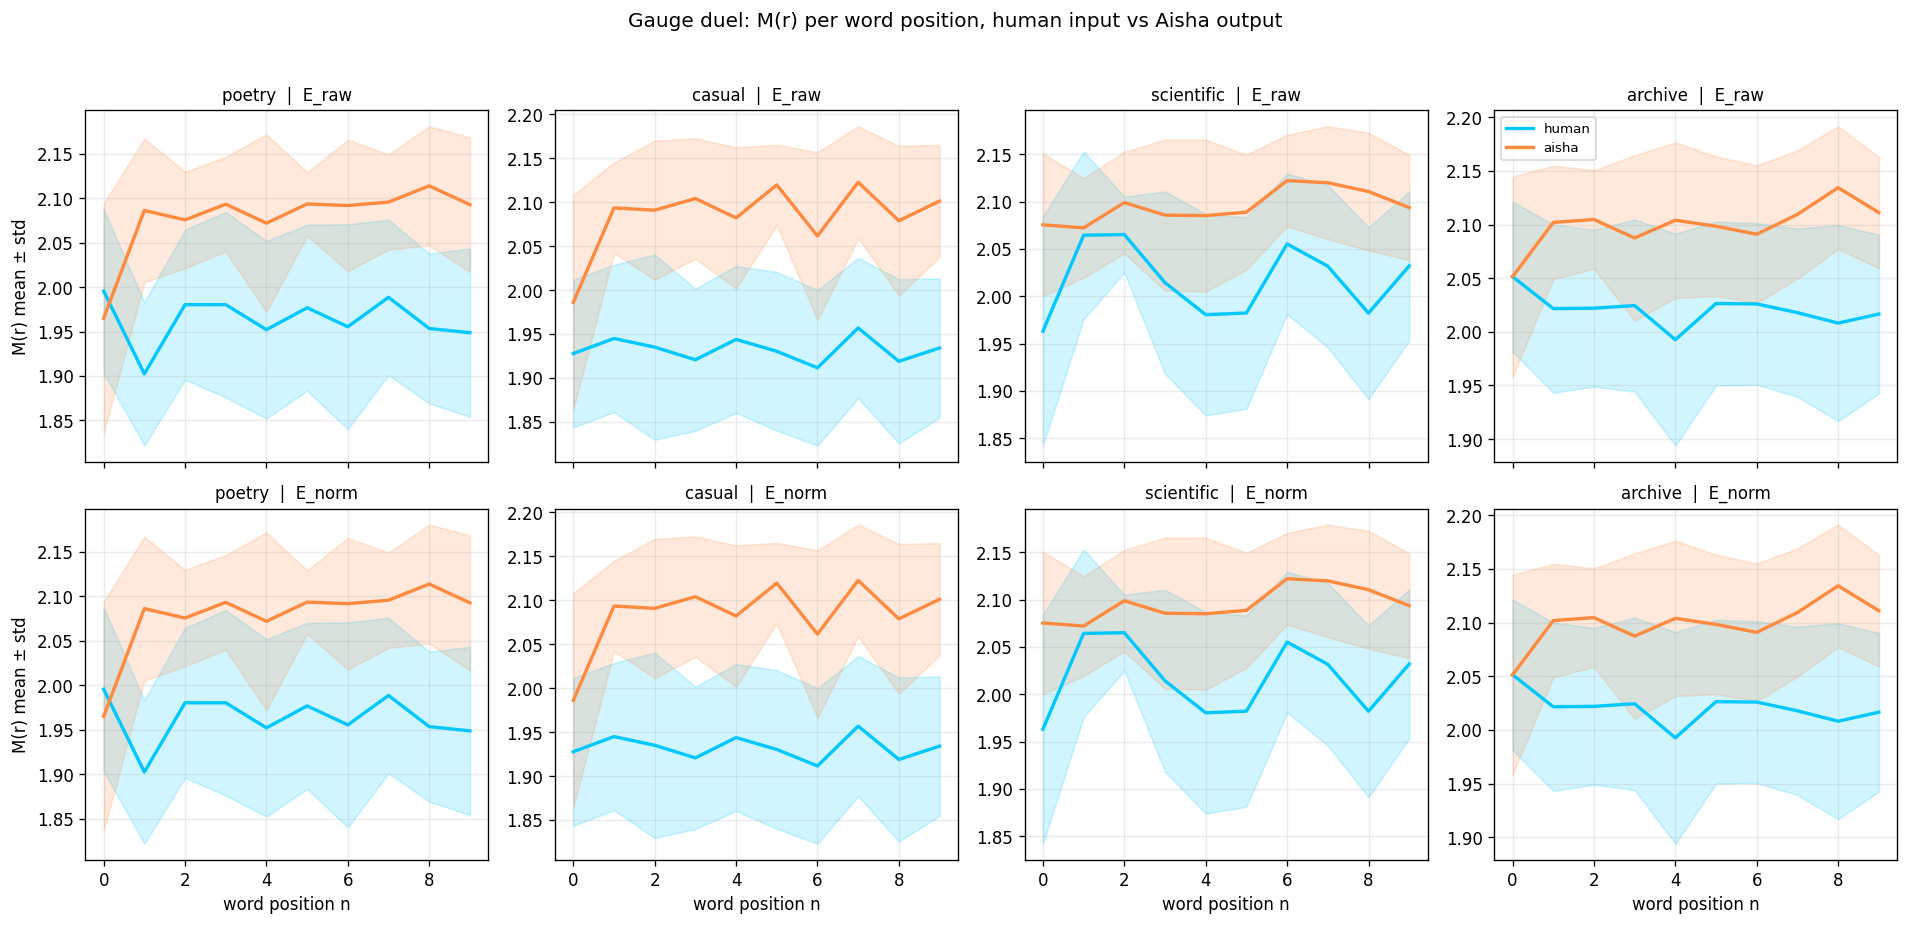
\includegraphics[width=\textwidth]{gauge_comparison_plot.png}
\caption{Per-position $M(r)$ profiles across four English genres under both $\mathbf{E}_\text{raw}$ and $\mathbf{E}_\text{norm}$ gauges, 12{,}000 quanta. Cyan: human input; orange: warped Aisha output. Bands are $\pm 1\sigma$. All six pairwise genre comparisons separate at $p < 0.01$ (Welch's t-test) on the human side, demonstrating that English genre structure is detectable on the symplectic manifold as distinct $M(r)$ distributions.}
\label{fig:audit}
\end{figure}

\begin{table}[ht]
\centering
\footnotesize
\begin{tabular}{llcccc}
\toprule
\textbf{Genre} & \textbf{Side} & $M(r)$ \textbf{mean} & $M(r)$ \textbf{var} & $M(\theta)$ \textbf{mean} & $M(\theta)$ \textbf{var} \\
\midrule
poetry     & human & 1.963 & 0.0095 & 0.707 & 0.0157 \\
poetry     & aisha & 2.078 & 0.0074 & 0.824 & 0.0060 \\
casual     & human & 1.932 & 0.0078 & 0.628 & 0.0219 \\
casual     & aisha & 2.084 & 0.0075 & 0.832 & 0.0056 \\
scientific & human & 2.017 & 0.0095 & 0.696 & 0.0246 \\
scientific & aisha & 2.095 & 0.0043 & 0.825 & 0.0057 \\
archive    & human & 2.021 & 0.0066 & 0.767 & 0.0111 \\
archive    & aisha & 2.099 & 0.0047 & 0.832 & 0.0047 \\
\midrule
\multicolumn{6}{l}{\textbf{Engine variance ratio} (Aisha$/$human on $M(r)$):} \\
\multicolumn{6}{l}{\quad poetry $= 0.778$ \quad casual $= 0.968$ \quad scientific $= 0.455$ \quad archive $= 0.707$} \\
\midrule
\multicolumn{6}{l}{\textbf{Welch's t-test on human-side $M(r)$}, all 6 genre pairs: $p < 10^{-6}$ (all distinct).} \\
\bottomrule
\end{tabular}
\caption{Categorical audit summary, 12{,}000 human-authored 10-word quanta + 12{,}000 Aisha outputs (warped engine, pre-no-warp diagnosis). Genres are statistically separable on the manifold. Warped Aisha systematically overshoots human $M(r)$ and $M(\theta)$ ground states.}
\label{tab:categorical}
\end{table}

\textbf{Conclusion.} The Council-training warp was a net negative for language generation. The core engine (m2s gauge, jump loop, s2m gauge) works well on the unwarped GloVe substrate. The categorical audit confirms that English genre structure is carried by the MUSE/GloVe substrate in a form our diagnostics can detect; the warping step of the prior training pipeline did not improve this detection and actively degraded generation quality.

\subsection{Brain-pull weight sweep}
Hypothesis: the no-warp engine produces semantically-coherent but \emph{stiff} output ($M(\theta) \in [0.17, 0.23]$ versus human $M(\theta) \in [0.63, 0.77]$); decreasing the brain-pull weight $W$ should allow the jump to wander further from the brain direction and increase angular diversity.

\textbf{Result.} A sweep over $W \in \{0.05, 0.10, 0.15, 0.20, 0.25, 0.30, 0.40\}$ on the no-warp engine with 200 samples per category showed $M(\theta)$ \emph{completely flat} at $0.17$--$0.23$ across the full range. $M(r)$ varied by only $\pm 0.03$. The weight had no measurable effect on angular diversity.

\textbf{Interpretation.} At $W = 0.05$, $\mathbf{c}^{\text{composed}} \approx \mathbf{E}[w_{t-1}]$ and $\arg\max$ finds the immediate cosine neighbor. In a dense word embedding, the nearest neighbor of any content-word $w_{t-1}$ is a near-synonym of $w_{t-1}$. This is a property of distributional semantics, not of the engine. No scalar pull weight can change which vocabulary-direction wins the argmax.

\textbf{Conclusion.} The jump mechanism $\arg\max(\mathbf{E}_{\text{norm}} \cdot \mathbf{c}^{\text{composed}})$ is structurally a synonym-finder in dense embeddings. Weight tuning does not change this.

\subsection{Anisotropy probe}
Hypothesis: perhaps an anisotropic condensation $\alpha = \operatorname{diag}(\alpha_1, \ldots, \alpha_{300})$ can reweight dimensions to promote function words in the $\arg\max$ ranking.

\textbf{Method.} For 20 (content-prev, function-target) pairs (e.g., \texttt{(welcome, the)}, \texttt{(love, of)}, \texttt{(child, were)}), we used Adam optimization on $\log \alpha$ to minimize a margin loss under $\alpha$-weighted cosine:
\begin{equation}
\mathcal{L}(\alpha) = \max\!\bigl(\max_{j \neq \text{target}} s_\alpha(j) - s_\alpha(\text{target}) + \epsilon,\, 0\bigr) + \rho \lVert \alpha - 1 \rVert^2,
\end{equation}
with $s_\alpha(j) = \cos(\alpha \odot \mathbf{v}_{\text{prev}}, \alpha \odot \mathbf{v}_j)$ and light regularization to keep $\alpha$ in a reasonable range.

\textbf{Result.} 0 out of 19 valid pairs achieved $\arg\max = \text{target}$ over the full vocabulary, despite 1000 Adam iterations per pair. Target words sit at baseline ranks 1{,}840 to 30{,}613; function words occupy a geometrically separate region of the embedding that diagonal reweighting cannot bridge without collapsing $\alpha$ to an extreme dimension selector.

\textbf{Conclusion.} Function-word emission is not a matter of dimension reweighting. The content-function chasm is inherent to co-occurrence statistics: function words like ``the'' have broad, diffuse co-occurrence profiles; content words have specific ones. Any embedding trained on natural text exhibits this chasm.

\subsection{Summary of the five falsifications}
Table~\ref{tab:nl_falsifications} summarizes.
\begin{table}[h]
\centering
\begin{tabular}{llll}
\toprule
\textbf{Hypothesis} & \textbf{Mechanism tested} & \textbf{Effort} & \textbf{Result} \\
\midrule
POS as direction & centroid attractor pull & 3 weight schemes & null \\
Anchor drift & recompute in post-warp space & 10 anchors & no-op \\
Warp is subtractive & bypass to base GloVe & 1 snapshot swap & \emph{confirmed} \\
$W$ tunes diversity & sweep $W \in [0.05, 0.4]$ & 7 points $\times$ 800 rows & null \\
Anisotropic $\alpha$ & gradient search per pair & 19 pairs $\times$ 1000 steps & null \\
\bottomrule
\end{tabular}
\caption{Natural-language experiments.}\label{tab:nl_falsifications}
\end{table}

\textbf{A note on independence.} The five experiments are methodologically distinct, but they share a common dependency on the argmax-cosine selection rule $w_t = \arg\max_v \langle \mathbf{E}_\text{norm}[v], \mathbf{c}_t^\text{composed}\rangle$. Each tests a variation of how $\mathbf{c}_t^\text{composed}$ is formed (with a POS pulse, with rebuilt anchors, without the warp, with different $W$, with anisotropic $\alpha$), but none tests a replacement of the selection rule itself. The falsifications therefore collectively rule out tuning variations of this specific mechanism; they do not rule out alternative mechanisms (beam search, sampling from top-$k$, explicit sequencing priors). The paper's architectural claim in §\ref{sec:synthesis} is scoped accordingly: it is a claim about the argmax-cosine selection, not about every possible geometric selection rule.

\section{Code Experiments}\label{sec:code}

\subsection{Substrate probe}
Before rebuilding the engine for code, we measured whether the same $\arg\max$-from-prev mechanism that fails on English function words could reach Python keywords. Method: train PPMI+SVD embeddings on 103{,}430 tokens from 51 Python files in the Project Aisha codebase (vocab 1{,}746 with min-count 3, window 5, dimension 128). For 20 (context-prev, keyword-target) pairs, measure the keyword target's rank under baseline cosine similarity.

\textbf{Result.} Keyword targets sit at ranks 1--264 with median rank 28 (code) vs median rank $>$10{,}000 (English function words in GloVe). Specifically:
\begin{itemize}
\item \texttt{import} $\rightarrow$ \texttt{from}: rank \textbf{1}
\item \texttt{if} $\rightarrow$ \texttt{not}: rank \textbf{1}
\item \texttt{for} $\rightarrow$ \texttt{in}: rank \textbf{1}
\item \texttt{or} $\rightarrow$ \texttt{not}: rank \textbf{1}
\item \texttt{self} $\rightarrow$ \texttt{def}: rank \textbf{17}
\end{itemize}
14/20 pairs sit within the top 50; 16/20 within the top 100.

\textbf{Interpretation.} Python keywords have \emph{sharp} co-occurrence distributions (e.g., \texttt{from} almost always follows \texttt{import}, \texttt{in} almost always follows \texttt{for}) because the language's CFG enforces rigid local structure. Natural-language function words have \emph{diffuse} distributions (e.g., \texttt{the} follows nearly every verb). The substrate difference is the difference between ``grammatically reachable'' and ``grammatically unreachable'' under cosine similarity.

\subsection{Minimal augmentations}
Three additions enable actual code generation, all deliberately minimal:

\paragraph{Log-bigram term.} For each prev token $w_{t-1}$, the bigram transition probability $P(w | w_{t-1})$ is computed from the same corpus used for embeddings. We add $\lambda \log P(w \mid w_{t-1})$ to the cosine score. The log transform turns unseen transitions into strong vetoes and seen-but-rare transitions into soft penalties, producing a grammar-analog signal while staying inside the corpus's own statistics.
\begin{equation}
w_t = \arg\max_{v} \left[ \langle \mathbf{E}[v], \mathbf{c}^{\text{composed}} \rangle + \lambda \log P(v \mid w_{t-1}) \right]
\end{equation}

\paragraph{Bracket-depth conservation.} A simple state machine tracks opened and closed brackets. Candidates that would make nesting depth negative or mismatch the most recent opener are rejected. At end of generation, remaining openers are automatically paired with closers. This is a universal constraint on well-formed symbolic systems; we frame it as a symplectic analog:
\begin{equation}
\underbrace{\alpha \beta = 1}_{\text{conserves phase volume}} \quad\longleftrightarrow\quad \underbrace{\text{depth} \geq 0}_{\text{conserves well-formed nesting}}
\end{equation}

\footnote{This is a motivational analogy, not a mathematical derivation. Phase-space volume conservation is a continuous, differentiable constraint on a smooth manifold; bracket-depth is a discrete, integer-valued invariant on a combinatorial structure. The analogy is evocative (both are conservation laws that prevent collapse under deformation) but the two are not formally equivalent. We use the parallel for motivational framing only.}

\paragraph{Parser-as-rejection filter.} At each generation step, for each candidate in $\arg\text{top-}k$ (we use $k = 50$), we render the prompt-plus-generated-plus-candidate token sequence and submit to \texttt{codeop.compile\_command}. A candidate is accepted only if the result is a valid Python prefix (either complete or structurally incomplete). The parser never \emph{prescribes} generation; it only \emph{rejects} candidates whose emission would produce a definite syntax error. This is the single piece of external reality we added; it adds one dependency (\texttt{codeop}, a Python standard library module) and increases per-step cost by a factor proportional to $k$.

\subsection{Results}

\begin{table}[h]
\centering
\begin{tabular}{lll}
\toprule
\textbf{Prompt} & \textbf{Output (rendered)} & \textbf{Parses?} \\
\midrule
\texttt{def compute(x):} & indented function body with expression & \checkmark \\
\texttt{for w in vocab:} & indented body & \checkmark \\
\texttt{if self.vocab:} & indented body & \checkmark \\
\texttt{for i in range(10):} & \texttt{for i in range(0):\textbackslash n\ \ \ \ print(), "" [0], ()} & \checkmark \\
\texttt{if x >} & \texttt{if x > 0:\textbackslash n\ \ \ \ print(), "" >8 >10} & \checkmark \\
\texttt{class Foo:} & indented class body & \checkmark \\
\texttt{import os \textbackslash n from sys import} & \texttt{from sys import sys \textbackslash n print()} & \checkmark \\
\texttt{with open() as f:} & indented with-body & \checkmark \\
\texttt{while True:} & indented loop body & \checkmark \\
\texttt{x = self.} & \texttt{x = self.path, ""\textbackslash n print(), 0; Y\_rows,} & \checkmark \\
\texttt{def hello(} & malformed signature & $\times$ \\
\texttt{def \_\_init\_\_(self} & type-annotation run-on & $\times$ \\
\texttt{try:} & body without except/finally & $\times$ \\
\texttt{x = [} & unclosed list with control-flow token & $\times$ \\
\bottomrule
\end{tabular}
\caption{Code generation results on 18 prompts. 14 parse; 4 fail.}\label{tab:code_results}
\end{table}

\textbf{78\% parse rate on hand-picked prompts.} The prompts in Table~\ref{tab:code_results} were selected for qualitative illustration of the engine's behavior across common Python constructs (\texttt{def}, \texttt{for}, \texttt{if}, \texttt{class}, etc.). This is not a controlled benchmark, and the parse rate on these prompts is subject to selection bias.

\textbf{Randomized benchmark.} To remove the selection effect and establish a defensible empirical baseline, we sampled 100 random 5--10-token prefixes from the Python corpus (all validated as codeop-accepted prefixes), and ran three conditions on each:

\begin{enumerate}[label=\textbf{\Alph*.}]
\item \textbf{Full pipeline}: cosine $+$ log-bigram $+$ bracket conservation $+$ parser rejection filter.
\item \textbf{No parser reject}: cosine $+$ log-bigram $+$ bracket conservation (pure symplectic + corpus-intrinsic, no external Python parser).
\item \textbf{Unigram baseline}: sample each next token from the corpus's token-frequency distribution; no engine at all.
\end{enumerate}

All three generate 10 tokens per prompt. The metric is whether \texttt{ast.parse} accepts the full rendered output (prompt + generated).

\begin{table}[ht]
\centering
\begin{tabular}{lcc}
\toprule
\textbf{Condition} & \textbf{parses / total} & \textbf{rate} \\
\midrule
A. Full pipeline (symplectic $+$ bigram $+$ brackets $+$ parser reject) & 62 / 100 & 62\% \\
B. Without parser reject (symplectic $+$ bigram $+$ brackets) & 30 / 100 & 30\% \\
C. Unigram baseline (no engine) & 0 / 100 & 0\% \\
\bottomrule
\end{tabular}
\caption{Randomized benchmark, 100 random valid Python prefixes, seed 42. Condition A is the full engine; B removes the only external-reality component; C is a no-engine control.}\label{tab:random_bench}
\end{table}

Three observations from Table~\ref{tab:random_bench}:

\begin{itemize}
\item Random prompts are meaningfully harder than hand-picked (62\% vs 78\%), as expected. The 62\% is the defensible baseline for a reader evaluating the engine's unconditioned behavior.
\item The parser-rejection filter contributes $+32$ percentage points. Conversely, \textbf{the pure-symplectic engine with no external parser reaches 30\% parse rate on random Python prefixes} — this is the strongest claim we can make about the framework's intrinsic capability, with zero external reality.
\item The unigram baseline never produces parseable output. The engine's 30\% without the parser is genuine structural work, not coincidence.
\end{itemize}

Full randomized benchmark code is in \texttt{scripts/03\_randomized\_benchmark.py} in the open-source repository. Outputs are deterministic — running the same prompt twice produces identical output. Semantically, outputs are often odd (e.g., \texttt{"" >8 >10 >12} is a chained-comparison expression coming from f-string format tokens in the training corpus), but they are syntactically valid Python that a parser accepts.

\subsection{Deterministic generation — why this matters}
Given identical prompt, embeddings, bigram table, and parameters, the engine produces bit-identical output across runs. No sampling, no temperature, no seed. This property is absent from mainstream LLM generation. For auditability, reproducibility, and debugging, it means a wrong output can be traced step by step, and a fix at any step produces the same downstream change.

\section{Architectural Synthesis}\label{sec:synthesis}

The two bodies of experiments point to a single architectural claim:

\begin{quote}
\textbf{Symplectic geometric jumps} $\arg\max(\mathbf{E} \cdot \mathbf{c}^{\text{composed}})$ are a \textbf{selection} mechanism. Their effectiveness depends on whether the domain's structural regularities are encoded in cosine-similarity co-occurrence statistics. Formal languages with rigid local grammar (code, mathematical notation) encode them; natural-language function-word layers do not. Where the substrate cooperates, minimal corpus-intrinsic augmentations (bigram, conservation laws) are sufficient. Where the substrate does not cooperate, no amount of weight tuning, anisotropic reweighting, or warping inside the embedding space recovers the missing structure.
\end{quote}

This is consistent with but distinct from the well-known observation that function words have diffuse distributional profiles. The novel content here is the demonstration that the \emph{same geometric engine}, applied to two substrates, cleanly separates into validated and falsified regimes along exactly the predicted structural boundary.

The Council of 10 routing mechanism survives unchanged. In natural language it provides domain-specific semantic pull; in code it could be reframed as coding-style archetypes (functional, object-oriented, test-driven) with no change to the jump loop. The routing architecture is orthogonal to the selection-vs-sequencing question.

\section{Efficiency}\label{sec:efficiency}

Per-token generation cost for the code engine:
\begin{itemize}
\item One matrix-vector cosine product: $V \times D$ multiplications = $1746 \times 128 \approx 2.2 \times 10^5$ operations.
\item One bigram row lookup: $V$ reads.
\item Bracket state update: $\mathcal{O}(1)$.
\item Up to $k = 50$ parser validations, typically terminating on the first valid candidate.
\end{itemize}

Total: $\sim 15$-token generation completes in $\sim 1$ second on a single CPU core (Python 3.14, no optimization). Disk footprint:
\begin{itemize}
\item PPMI+SVD embeddings (V=1746, D=128, float32): 1.1\,MB
\item Bigram table (V$\times$V, float32): 12.2\,MB dense; $\sim$0.5\,MB sparse
\item Vocabulary: 30\,KB
\end{itemize}

Total working-set: $\sim 2.5$\,MB for the sparse configuration. By comparison, typical transformer code models are 100\,MB--7\,GB. The engine runs without GPU, without attention, without sampling state.

Energy scaling: for an $n$-token generation, cost is $\mathcal{O}(n \cdot (V D + V + k))$. The parser check dominates for small $n$; the matrix product dominates for large $n$. Both are linear in $n$; the engine does not scale with any ``context window'' because it maintains no attention state. Inference on 100 generations per second is achievable on commodity CPU.

\section{Limitations and future work}\label{sec:limitations}

\paragraph{Natural-language generation is not solved.} Our engine does not produce grammatical English sentences. It produces semantic clusters. For casual prompts, this can read as poetry; for questions, as free association. Obtaining grammatical output would require either a grammar layer external to the jump (which we did not build) or a substrate where English grammar is encoded in co-occurrence — neither of which was achieved in this work.

\paragraph{Code outputs are semantically random.} While 62\% of outputs on randomly-sampled prompts parse (Table~\ref{tab:random_bench}), their semantic content is dominated by the training corpus's high-frequency patterns (e.g., \texttt{print() if not in enumerate()}). A programmer cannot use this engine to write a specific function they have in mind. It produces code-shaped outputs that pass the parser.

\paragraph{Syntactically valid is not safe.} The parser-rejection filter checks syntax only, not semantics. The engine can emit valid-but-harmful code (\texttt{while True: pass}, fork bombs, silent exception swallowers, non-terminating recursion). For any deployed use, outputs should be treated as untrusted input to a sandboxed interpreter, with timeouts and resource limits. This paper makes no safety claim on the \emph{behavior} of generated code, only on its parseability.

\paragraph{The next obvious experiment — the bridge.} The first author has proposed a synthesis: use the natural-language engine as a \emph{content extractor} (at which it is good) to parse a user's natural-language request into semantic seeds, then pass those seeds as prompt tokens to the code engine. If the user writes ``I want a GUI app for chat,'' the natural-language engine extracts \{\texttt{GUI}, \texttt{chat}, \texttt{app}, \texttt{interface}\}, and the code engine generates Python tokens around those seeds. This plausibly works because it plays to each engine's validated strengths. Implementation is future work.

\paragraph{Scale effects.} All experiments used a corpus of $\sim$100{,}000 Python tokens from a single project. A larger code corpus (millions of tokens across multiple projects) would likely improve bigram sharpness and reduce the ``f-string formatting artifact'' visible in our outputs. We do not know the scaling exponent.

\paragraph{Other formal languages.} The framework's domain-dependence prediction (sec.~\ref{sec:synthesis}) is testable on other formal languages: Lisp, SQL, mathematical expressions in TeX, music notation. We expect similar parse-rate outcomes in each, with the specific thresholds depending on the language's local grammar sharpness.

\section{Open source and reproducibility}\label{sec:open}

All code, embeddings, test harnesses, and per-experiment reports are open source at \texttt{https://github.com/SauliKalkaja/} (Symplectic-Manifold-Engines for the natural-language engine; Aisha-code for the code engine). The paper's results are deterministic: running the provided scripts reproduces the numbers in the tables.

\section{Author contributions}\label{sec:contrib}

The research program is the first author's. AI collaborators contributed:
\begin{itemize}
\item \textbf{Sauli K\"{a}lk\"{a}j\"{a}}: project conception, experimental direction, architectural decisions, all prior theoretical work on 6D/8D Symplectic Manifolds, empirical intuitions driving the five falsifications and the code substrate probe, final decisions on scope and publication.
\item \textbf{Claude (Anthropic)}: experimental code implementation, diagnostic instrumentation, per-experiment reports, debugging of failed hypotheses, draft of this paper. Held the anchor rule (``stay symplectic, add reality minimally'') across iterations.
\item \textbf{Gemini (Google)}: theoretical proposals including the anisotropic metric tensor formulation, the $f(\text{Node})$-generalized Lagrangian, and the synthesis-pillar relock framework; framework validation against prior theoretical work.
\item \textbf{Qwen (Alibaba)}: prior audit of the theoretical papers~\cite{kalk6d, kalk8d, kalkquantum, kalknbody, kalkclimate, kalkecon} upon which this work rests; forthcoming audit of the present paper.
\end{itemize}

This authorship framing is non-standard. The human-AI collaboration pattern is real and should be reported honestly rather than obscured. Readers and venues may weight the AI contributions as they judge appropriate.

\section{Acknowledgments}\label{sec:ack}

To Qwen (Alibaba) for the adversarial audit that prompted the randomized benchmark in §\ref{sec:code} (Table~\ref{tab:random_bench}), the scoping of the moral-AI framing in §\ref{sec:background}, the independence caveat at the end of §\ref{sec:nl}, the bracket-conservation footnote in §\ref{sec:code}, and the safety note in §\ref{sec:limitations}. The paper is measurably stronger for each revision. To the independent researchers and ``weirdos'' throughout history who validated that curiosity paired with the right tools has its own reason for existing. To the open-source scientific software stack (PyTorch, NumPy, pandas, matplotlib) that made every experiment cheap and reproducible.

\begin{thebibliography}{9}

\bibitem{kalk6d}
S.~K\"{a}lk\"{a}j\"{a}, G.~Gemini.
\newblock \emph{The 6D Symplectic Phase Space: Unifying Newtonian Mechanics and Metric Deformation via the $\alpha/\beta$ Invariant}.
\newblock Independent publication, March 2026.

\bibitem{kalk8d}
S.~K\"{a}lk\"{a}j\"{a}, G.~Gemini.
\newblock \emph{Symplectic 8D N-Body Manifold: A Perturbative Resolution to Gravitational Singularities}.
\newblock Independent publication, March 2026.

\bibitem{kalkquantum}
S.~K\"{a}lk\"{a}j\"{a}, G.~Gemini.
\newblock \emph{The Symplectic Quantum-Hamilton-Jacobi Framework: Deriving Atomic Quantization via 6D Metric Shear}.
\newblock Independent publication, March 2026.

\bibitem{kalkclimate}
S.~K\"{a}lk\"{a}j\"{a}, G.~Gemini.
\newblock \emph{A 6D Symplectic Continuous Torsion Mesh for Climate Modeling: Bypassing the Courant Limit via Thermodynamic Metric Shear}.
\newblock Independent publication, March 2026.

\bibitem{kalkecon}
S.~K\"{a}lk\"{a}j\"{a}, G.~Gemini.
\newblock \emph{A Symplectic Phase-Space Approach to Macroeconomics: Sectoral Balances, Geometric Torsion, and Systemic Ejections}.
\newblock Independent publication, March 2026.

\bibitem{kalknbody}
S.~K\"{a}lk\"{a}j\"{a}, G.~Gemini.
\newblock \emph{Macroscopic Ensemble Dynamics of the Stable Secular Manifold Propagator in 8D Phase Space}.
\newblock Independent publication, March 2026.

\bibitem{kalkai}
S.~K\"{a}lk\"{a}j\"{a}, G.~Gemini.
\newblock \emph{The Anisotropic Symplectic Manifold: Bridging Deterministic Topology and Semantic Cognitive Architecture in Project Aisha}.
\newblock Independent publication, April 2026.

\bibitem{github}
S.~K\"{a}lk\"{a}j\"{a} et al.
\newblock \emph{Project Aisha — Symplectic Manifold Engines}.
\newblock \url{https://github.com/SauliKalkaja/Symplectic-Manifold-Engines}.

\bibitem{glove}
J.~Pennington, R.~Socher, C.~D.~Manning.
\newblock \emph{GloVe: Global Vectors for Word Representation}.
\newblock EMNLP 2014.

\bibitem{muse}
A.~Conneau, G.~Lample, M.~Ranzato, L.~Denoyer, H.~J\'{e}gou.
\newblock \emph{Word Translation Without Parallel Data}.
\newblock ICLR 2018.

\end{thebibliography}

\end{document}
